% Lecture file created by newnote
% Class: Models of Theoretical Physics
% Professor: Azaele Sandro
% Date: 2025-10-17
\lecture{8}{Introduction to Stochastic Processes}{2025-10-17}
\pagelayout{margin}
% --- Start writing here ---

\section{Introduction to Stochastic Processes}
We will present basic results from the theory of stochastic processes. Rigorous definitions and proofs need notions of measure theory that we do not introduce nor assume. therefore, this introduction will necessarily be non-rigorous, with some looseness in the definitions and some inaccuracies in the proofs. There are many books which can give you the mathematical rigor that is necessary for obtaining a full understanding of stochastic processes. These notes, instead, wish to provide enough awareness to make you able to use the tools in applied problems (in physics, biology, finance...).

In the following we will connect the diffusion equation to the most important continuous stochastic process: the Brownian motion (or Wiener Process). This is the basis for building up stochastic differential equations whose solutions have continuous trajectories. These are crucial for defining stochastic models that will be used in several fields of physics.

Useful books:
\begin{itemize}
    \item "Intro. to Stoch. Calculus with Applic.", F.C. Klebaner, Imperial P.
    \item "An Introd. to SDEs", Lawrence C. Evans, AMS
    \item "Stoch. Proc. and Applications", G. A. Pavliotis, Springer
    \item "Stoch. Methods", C. Gardiner, Springer
    \item "Stoch. Diff. Eq.", B. Oksendal, Springer
    \item "Stoch. proc. in Physics and chemistry", N.G. van Kampen.
\end{itemize}

\subsection*{Example: Tossing a coin}
Let's assume that we toss a coin 3 times (heads $\rightarrow 0$, tails $\rightarrow 1$) and we ask: what is the sum of the 3 tosses? We define a function from the sample space (the realization) to the state space (what we measure)
$Y: \Omega=\{\omega_1=(0,0,0), \omega_2=(0,0,1) \ldots \omega_8=(1,1,1)\} \longrightarrow E=\{y_1=0, y_2=1, y_3=2, y_4=3\}$
and introduce probabilities $\mathbb{P}: \Omega \rightarrow[0,1]$ s.t. $\sum_{\omega} P(\omega)=1$; we define $P_{i}=\sum_{\omega: Y(\omega)=y_{i}} \mathbb{P}(\omega)=P\left(Y=y_{i}\right)$. More generally, we can define probabilities for all sets of type $Y^{-1}(B) \subseteq \Omega$, for $B \subseteq E$. This means that $Y$ is a measurable function and this defines a random variable.
When $\Omega$ is finite, $Y(\Omega)$ is finite and we can always define a random variable as before. We can also define the expectation as
\begin{DispWithArrows}
    E(Y)=\sum_{\omega \in \Omega} Y(\omega) \mathbb{P}(\omega)=\sum_{i=1}^{4} y_{i} P\left(Y=y_{i}\right)=\sum_{i=1}^{4} y_{i} P_{i}
\end{DispWithArrows}
When $\Omega$ is an uncountable set, the definition of r.v. needs much care, because we have to make sure that $x$ is still a measurable function. In simple terms $x$ is a real-valued random variable when we can assign probabilities to sets (called events) of the form {x \leq c} and {a<x \leq b} for $x, a, b \in \mathbb{R}$.
\begin{figure}[H]
    \centering
    
\includegraphics[width=0.5\textwidth]{2025_10_17_79731b7d4e7690819b81g-02}
\end{figure}
More precisely, a random variable is a measurable function for which the preimage of any Borel set in $\mathbb{R}$ is a measurable set in $\Omega$.

\subsection*{Definition of stochastic process}
A stochastic process is a collection of random variables {x(t, $\omega$), t \in T, $\omega$ \in $\Omega$}, where T is an ordered set ("time") (it can be either discrete, $T=\mathbb{Z}_{+}$, or continuous, $T=\mathbb{R}^{+}$). For each fixed time $t \in T, x(t, \omega)$ indicates a random variable from $\Omega$ (rigorously, from the probability space $(\Omega, \mathcal{F}, \mathbb{P})$ ) to $E$ (rigorously, $E$ is a measurable space equipped with a $\sigma$-algebra; for instance, $E=\mathbb{R}^{d}$ and the $\sigma$-algebra is the one of Borel sets; we need a "filtration" as well).
$\Omega$ is the common sample space, $E$ is the state space of the process.
For each fixed $\omega \in \Omega, x(t, \omega)$ is a function of time $t$ that is called a sample path or a stochastic realization of the process. We will usually omit the $\omega$-dependence, i.e., we write $x(t)$.

\subsection*{Examples:}
\begin{enumerate}
    \item Let $E=\{0,1,-1\}$ be the state space of a stoch-proc $x$ and let $T=\{0,1,2,3\}$ be the (discrete) time. There are then $3^{4}$ sample paths, thus $|
\Omega|=3^{4}=81$.
    \begin{figure}[H]
        \centering
        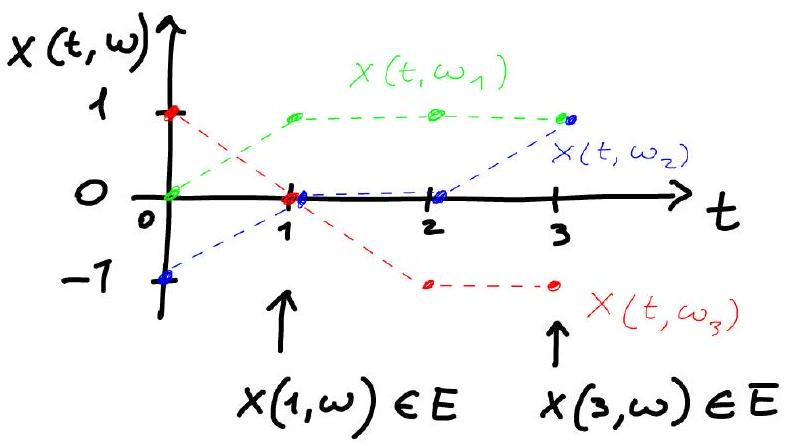
\includegraphics[width=0.5\textwidth]{2025_10_17_79731b7d4e7690819b81g-03}
    \end{figure}
    In this example we can enumerate all the 81 trajectories. This is not possible if $E$ is an uncountable set.
    \item The random walk process in discrete time has $E=\mathbb{Z}$ (position) and $T=\mathbb{N}$ (time), thus $x(t, \omega)$ indicates a stochastic realization (or trajectory) as a function of time $t$.
    \begin{figure}[H]
        \centering
        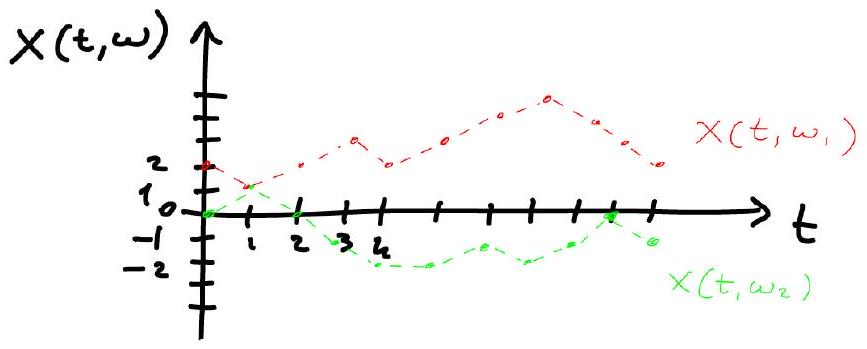
\includegraphics[width=0.5\textwidth]{2025_10_17_79731b7d4e7690819b81g-03(1)}
    \end{figure}
    Here we get infinitely countable trajectories ($|
\Omega|=|\mathbb{Z}|^{\mathbb{N}}$)
    \item The position of a Brownian particle is described by the Brownian process for which $T=\mathbb{R}^{+}$ and $E=\mathbb{R}$ and one sample path is $x(t, \omega)$
    \begin{figure}[H]
        \centering
        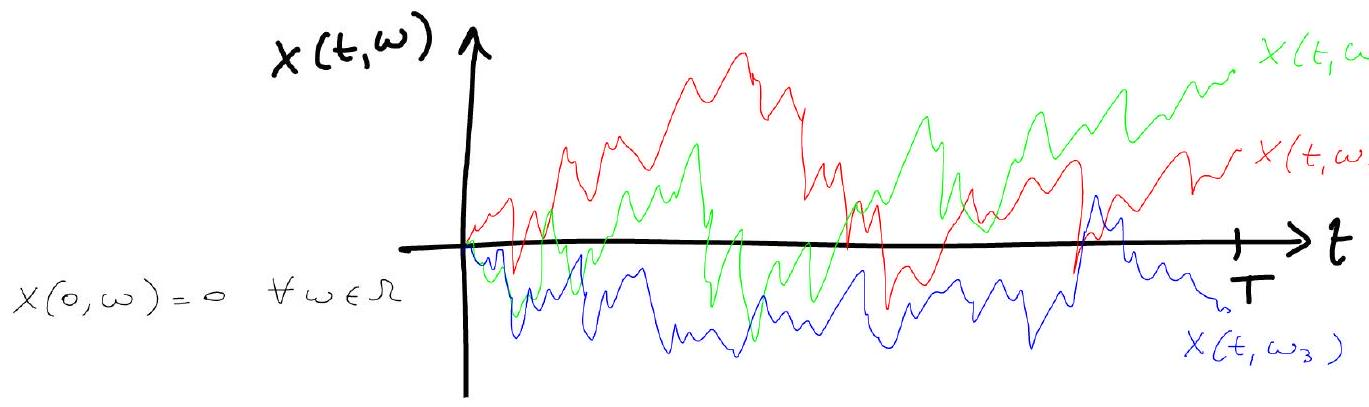
\includegraphics[width=0.5\textwidth]{2025_10_17_79731b7d4e7690819b81g-03(2)}
    \end{figure}
    here every path is a continuous function of time $x(t, \omega) \in C^{0}([0, T])$
\end{enumerate}
In the following we will omit $\omega$ and we will simply write $x(t)$, because what we "observe" is the value $x \in E$ at some time $t$ and not $
\Omega$.

Notice that in these examples we have not defined a prob. measure, which is not needed for defining a random variable.

One of the most important stochastic processes is the Brownian process/motion or Wiener process.
This can be used to describe the motion of a heavy particle in a fluid made of light particles, which collide with it randomly. For the time being, we will not look into how good this process is for empirical Brownian particles.

\subsection*{Brownian motion (or Wiener process)}
A standard Brownian motion in 1-d, $B(t)$, is a real-valued stoch. process ($E=\mathbb{R}, T=\mathbb{R}^{+}$) for which
(A) $B(0)=0$ (a.s. , namely, Prob. {B(0)=0}=1)
(B) For any $0 \leqslant s<t<\infty, B(t)-B(s)$ is normally distributed, that is $B(t)-B(s) \sim N(0, t-s)=\frac{1}{\sqrt{2 \pi(t-s)}} e^{-\frac{\Delta x^{2}}{2(t-s)}}$ (mean 0 and variance $t-s$)
(C) For all times $0=t_{0}<t_{1}<t_{2}<\ldots<t_{n}$ the increments $\Delta B_{i}:=B\left(t_{i}
ight)-B\left(t_{i-1}
ight)$ are independent (of each other)

Some important properties:
\begin{enumerate}
    \item Stationarity of increments: notice that, if we write $t=s+\Delta t$, then from (B) we get
    \begin{DispWithArrows}
        B(s+\Delta t)-B(s) \sim N(0, \Delta t)
    \end{DispWithArrows}
    which means that the distribution of $B(s+\Delta t)-B(s)$ does not depend on $s$. This means that the increments are not only independent, but also stationary, namely they depend only on $\Delta t: \Delta B=B(s+\Delta t)-B(s) \sim B(\Delta t)$.

    Since $\operatorname{Var}[B(\Delta t)]=\Delta t$, we expect that $|
\Delta B|=|B(\Delta t)| \simeq \sqrt{\Delta t}$ as $\Delta t \rightarrow 0^{+}$. This will be crucial in the future, in many calculations.
    \item Connection with the diffusion equation

    We have seen that the fundamental solution of the diffusion eq. ($D=1$)
    \begin{DispWithArrows}
        \left\{\begin{array}{cc}
        \partial_{t} w(x, t)=\frac{1}{2} \partial_{x}^{2} w(x, t) & x \in \mathbb{R}, t>t_{0} \\
        w(x, t_{0})=\delta\left(x-x_{0}
ight) & t=t_{0}
        \end{array}\right.
    \end{DispWithArrows}
    is the propagator of the Brownian motion:
    \begin{DispWithArrows}[tag=1]
        w\left(x, t \mid x_{0}, t_{0}
ight)=\frac{1}{\sqrt{2 \pi\left(t-t_{0}
ight)}} e^{-\frac{\left(x-x_{0}
ight)^{2}}{2\left(t-t_{0}
ight)}}
    \end{DispWithArrows}
    which is the one we use in (B). So from time to time the process evolves with the propagator (1) and with stationary independent increments.
    \item Correlation function

    The average will be indicated either with $\langle\cdots\rangle$ or with $\mathbb{E}(\cdots)$. Let $0 \leqslant s \leqslant t:$ from (B) $\mathbb{E}[B(s)]=0, \mathbb{E}\left[B(s)^{2}
ight]=s$. Then
    \begin{DispWithArrows}
        \begin{aligned}
        \mathbb{E}[B(t) B(s)] & =\mathbb{E}[(B(s)+B(t)-B(s)) B(s)]=\
        & =\mathbb{E}\left[B(s)^{2}+(B(t)-B(s)) B(s)\right]=\
        & =\mathbb{E}\left[B(s)^{2}\right]+\mathbb{E}[(B(t)-B(s)) B(s)]=\
        & =s+\mathbb{E}[(B(t)-B(s))] \mathbb{E}[B(s)]=s
        \end{aligned}
    \end{DispWithArrows}
    Thus for $s, t \geqslant 0$
    \begin{DispWithArrows}[tag=2]
        \mathbb{E}[B(t) B(s)]=\min (t, s)
    \end{DispWithArrows}
    Exercises:
    i) (Ornstein-Uhlenbeck process). Define $V(t)=e^{-t} B\left(e^{2 t}
ight)$ where $B(t)$ is a Brownian process. Show that $\mathbb{E}[V(t)]=0$ and $\mathbb{E}[V(t) V(s)]=e^{-|t-s|}$.
    ii) (Brownian bridge). Define $V(t)=B(t) - (t/T)B(T)$ for any $t \in[0, T]$, where $B(t)$ is a Brownian process. Show that $\mathbb{E}[V(t)]=0$ and $\mathbb{E}[V(t) V(s)]=\min(t,s) - ts/T$ for any $t, s \in[0, T]$.
    iii) Show that $\mathbb{E}\left[e^{i \lambda B(t)}\right]=e^{-\frac{\lambda^{2} t}{2}}$ for $t \geqslant 0, B(t)$ B.m.
    iv) With the help of the Law of large numbers and $B(t)=\sum_{i=1}^{t/\Delta t} \Delta B_{i}$, show that $\lim _{t \rightarrow \infty} \frac{B(t)}{t}=0$.
    \item Rescaling. The process $z(t)=\frac{1}{\sqrt{c}} B(c t), c>0$, is a Brownian motion that is distributed like $B(t)$, another Brownian motion. (Verify $(A),(B)$ and $(C)$ ). Also:
    \begin{DispWithArrows}
        \mathbb{E}\left[e^{i \lambda z(t)}\right]=\mathbb{E}\left[e^{i \lambda \frac{1}{\sqrt{c}} B(c t)}\right]=e^{-\frac{\lambda^{2}}{2 c} t c}=e^{-\frac{\lambda^{2} t}{2}}=\mathbb{E}\left[e^{i \lambda B(t)}\right]
    \end{DispWithArrows}
    \item Inversion. The process $z(t)=t B\left(\frac{1}{t}
ight)$ for $t>0$ and $z(0)=0$ is distributed like $B(t)$, another B.m.
    \begin{DispWithArrows}
        \mathbb{E}\left[e^{i \lambda z(t)}\right]=\mathbb{E}\left[e^{i \lambda t B\left(\frac{1}{t}
ight)}\right]=e^{-\frac{\lambda^{2}}{2} t^{2} \cdot \frac{1}{t}}=e^{-\frac{\lambda^{2} t}{2}}=\mathbb{E}\left[e^{i \lambda B(t)}\right]
    \end{DispWithArrows}
    Notice that $\lim _{t \to \infty} \frac{z(t)}{t}=\lim _{t \to \infty} B\left(\frac{1}{t}
ight)=0$ as in (iv).
    \item Time reversal. Define $z(t)=B(T)-B(T-t)$ for any $t \in[0, T]$. Then $Z(t)$ and $B(t)$ have the same distrib.
\end{enumerate}

\subsection*{Properties of the trajectories of the Brownian motion}
These are hard to prove rigorously, but somehow easy to guess. Let's consider the ratio $rac{\Delta B}{(\Delta t)^{\alpha}}$ where $\Delta t=t_{2}-t_{1}>0, \alpha>0$ and $\Delta B=B\left(t_{2}
ight)-B\left(t_{1}
ight)$. What happens to this ratio as $\Delta t \rightarrow 0^{+}$? Take some $k \in \mathbb{R}^{+}$:
\begin{DispWithArrows}[tag=3]
    \begin{aligned}
    P\left(\left|\frac{\Delta B}{\Delta t^{\alpha}}\right| \leqslant k\right) & =P\left(|
\Delta B| \leqslant k \Delta t^{\alpha}\right)=\int_{-k(\Delta t)^{\alpha}}^{k(\Delta t)^{\alpha}} d x \frac{e^{-\frac{x^{2}}{2 \Delta t}}}{\sqrt{2 \pi \Delta t}}}=\
    & =\frac{2}{\sqrt{2 \pi \Delta t}} \int_{0}^{k(\Delta t)^{\alpha}} d x e^{-\frac{x^{2}}{2 \Delta t}}=\frac{2}{\sqrt{2 \pi}} \int_{0}^{k(\Delta t)^{\alpha-1 / 2}} d z e^{-z^{2} / 2}
    \end{aligned}
\end{DispWithArrows}
Here are the consequences:
\begin{enumerate}
    \item $0<\alpha<\frac{1}{2}$, as $\Delta t \rightarrow 0^{+}, \quad P\left(\left|\frac{\Delta B}{\Delta t^{\alpha}}\right| \leqslant k\right) \rightarrow 1$ regardless of $k$. This tells us that as $|t-s| \rightarrow 0^{+}$
    \begin{DispWithArrows}
        $|B(t)-B(s)| \leqslant \text { const }|t-s|^{\alpha}$
    \end{DispWithArrows}
    which means that Brownian trajectories are Hölder continuous for any $0<\alpha<\frac{1}{2}$. This can be proven rigorously.
    \item $\alpha=1$ (or $\frac{1}{2}<\alpha \leqslant 1$), as $\Delta t \rightarrow 0^{+}, P\left(\left|\frac{\Delta B}{\Delta t}\right| \leqslant k\right) \rightarrow 0 \quad \forall k \in \mathbb{R}^{+}$
\end{enumerate}
This tells us that the Brownian trajectories are nowhere differentiable. This is expected because if $|
\Delta B| \sim \sqrt{\Delta t}$, then $\frac{|
\Delta B|}{\Delta t} \sim \frac{1}{\sqrt{\Delta t}}$ and hence $\lim _{\Delta t \rightarrow 0^{+}} \frac{|
\Delta B|}{\Delta t} \rightarrow \infty$.
This is related to the fact that B.m. has no memory of the past (see the Markov property below).

We can add a drift $\mu$ and change the diffusion coefficient of a Brownian motion with no difficulty. We define a Brownian motion with drift $\mu$ and variance $D$ the process
\begin{DispWithArrows}[tag=4]
    x(t)=x_{0}+\mu t+\sqrt{2D} B(t)
\end{DispWithArrows}
Verify that $\mathbb{E}[x(t)]=x_{0}+\mu t$ and $\operatorname{Var}[x(t)] \equiv \mathbb{E}\left[(x(t)-\mathbb{E}[x(t)])^{2}\right]=2Dt$. Notice that $x(t)$ satisfies the stochastic differential equation:
\begin{DispWithArrows}[tag=5]
    d x(t)=\mu d t+\sqrt{2D} d B(t)
\end{DispWithArrows}
How to simulate a very simple SDE (including B.m.) We wish to generate a path of eq. (5), starting from $x(0)=x_{0}$. Because $\Delta B \sim B(\Delta t) \sim \sqrt{\Delta t} B(1)$ for finite times $t_{0}=0<t_{1} \cdots <t_{n-1}<t_{n}$ we can write (5) as ($\Delta t=t_{i}-t_{i-1}$)
\begin{DispWithArrows}[tag=6]
    \begin{aligned}
    x\left(t_{i}\right) & =x\left(t_{i-1}
ight)+\mu \Delta t+\sqrt{2D \Delta t} \varepsilon_{i} \\
    x(0) & =x_{0}
    \end{aligned} \quad i=1,2, \ldots, n
\end{DispWithArrows}
where $\varepsilon_{i} \sim N(0,1)$. Notice that we use a sequence of $n$ independent and identically distributed random variables {$\varepsilon_{i}$} drawn from $N(0,1)$ because at every time step we add a random value that is independent of all values that were calculated before (indep. of $x, t, \mu, D \ldots$). Of course, $\mu=0, D=1/2$ and $x_{0}=0$ generate a standard Brownian motion as defined in $(A),(B)$ and $(C)$.

\subsection*{Markov processes}
Let us focus on a stochastic process for which we can take a set of ordered times, i.e. $t_{0}<t_{1}<t_{2} \cdots<t_{n}$ and there exists a conditional prob. density funct. at time $t_{n}$, namely $p_{1|n-1}
\left(x_{n}, t_{n} 
\mid x_{n-1}, t_{n-1} ; \ldots ; x_{1}, t_{1} ; x_{0}, t_{0}
ight)$.
This PDF tells us what is the prob. of observing $x_{n}$ at time $t_{n}$, if we know what happened to the process at previous times; we really know the actual values that occurred, not only their probabilities. This is quite a lot of information and basically it means that, if we want to make a prediction on what is going to happen in the future, we have to know all that happened in the past. However, in some situations the effect of the past can be neglected. In particular, if it happens that for any $n=1,2 \ldots$
\begin{DispWithArrows}[tag=7]
    $p_{1|n-1}
\left(x_{n}, t_{n} 
\mid x_{n-1}, t_{n-1} ; \ldots ; x_{1}, t_{1} ; x_{0}, t_{0}
ight)=p_{1|1}
\left(x_{n}, t_{n} 
\mid x_{n-1}, t_{n-1}
ight)$
\end{DispWithArrows}
Then we say that the stochastic process is a Markov process. This means that predictions at time $t_{n}$ only depend on what happened at time $t_{n-1}$ and not on the whole history of the process. The pdf $p_{1|1}$ is called transition probability or propagator.

A Markov process can be fully defined by two functions: the propagator $p_{1|1}$ and the initial distribution $p_{1}
\left(x_{0}, t_{0}
ight)$.

Indeed the 3-point joint PDF for a Markov process is ($t_{0}<t_{1}<t_{2}$):
\begin{DispWithArrows}[tag=8]
    \begin{aligned}
    P_{3}
\left(x_{2} t_{2} ; x_{1} t_{1} ; x_{0} t_{0}
ight) & =P_{1|2}
\left(x_{2} t_{2} 
\mid x_{1} t_{1} ; x_{0} t_{0}
ight) P_{2}
\left(x_{1} t_{1} ; x_{0} t_{0}
ight)=\
    & =p_{1|1}
\left(x_{2} t_{2} 
\mid x_{1} t_{1}
ight) P_{2}
\left(x_{1} t_{1} ; x_{0} t_{0}
ight) \\
    & =P_{1|1}
\left(x_{2} t_{2} 
\mid x_{1} t_{1}
ight) P_{1|1}
\left(x_{1} t_{1} 
\mid x_{0} t_{0}
ight) P_{1}
\left(x_{0} t_{0}
ight)
    \end{aligned}
\end{DispWithArrows}
Therefore we can find iteratively
\begin{DispWithArrows}[tag=9]
    p_{n}
\left(x_{n} t_{n} ; x_{n-1} t_{n-1} ; \ldots ; x_{1} t_{1} ; x_{0} t_{0}
ight)=\prod_{i=1}^{n} p_{1|1}
\left(x_{i} t_{i} 
\mid x_{i-1} t_{i-1}
ight) p_{1}
\left(x_{0} t_{0}
ight)
\end{DispWithArrows}
this property makes Markov processes much more amenable to analytical calculations than non-Markov ones.

\subsection*{The Chapman-Kolmogorov equation}
Not all functions can be used as propagators for Markov processes, nor an initial distribution $p_{1}$ can be arbitrary. These two functions must satisfy two identities, one of which is the C-K. equation.

From the L.H.S. of eq. (8), if we integrate wrt $x_1$,
\begin{DispWithArrows}
    $\int d x_{1} p_{3}
\left(x_{2} t_{2} ; x_{1} t_{1} ; x_{0} t_{0}
ight)=p_{2}
\left(x_{2} t_{2} ; x_{0} t_{0}
ight)$
\end{DispWithArrows}
from the R.H.S., instead
\begin{DispWithArrows}
    $=\int d x_{1} p_{1|1}
\left(x_{2} t_{2} 
\mid x_{1} t_{1}
ight) p_{1|1}
\left(x_{1} t_{1} 
\mid x_{0} t_{0}
ight) p_{1}
\left(x_{0} t_{0}
ight)$
\end{DispWithArrows}
but $p_{2}
\left(x_{2} t_{2} ; x_{0} t_{0}
ight)=p_{1|1}
\left(x_{2} t_{2} 
\mid x_{0} t_{0}
ight) p_{1}
\left(x_{0} t_{0}
ight)$, because of the Markov property, so
\begin{DispWithArrows}[tag=10]
    $p_{1|1}
\left(x_{2} t_{2} 
\mid x_{0} t_{0}
ight) p_{1}
\left(x_{0} t_{0}
ight)=\int d x_{1} p_{1|1}
\left(x_{2} t_{2} 
\mid x_{1} t_{1}
ight) p_{1|1}
\left(x_{1} t_{1} 
\mid x_{0} t_{0}
ight) p_{1}
\left(x_{0} t_{0}
ight)$
\end{DispWithArrows}
hence, for any $t_{2}>t_{1}>t_{0}$
\begin{DispWithArrows}[tag=11]
    $p_{1|1}
\left(x_{2} t_{2} 
\mid x_{0} t_{0}
ight)=\int d x_{1} p_{1|1}
\left(x_{2} t_{2} 
\mid x_{1} t_{1}
ight) p_{1|1}
\left(x_{1} t_{1} 
\mid x_{0} t_{0}
ight)$
\end{DispWithArrows}
this is the Chapman-Kolmogorov equation (actually, identity), which must be satisfied by any propagator/transition probab. If we further integrate eq. (10) w.r.t. $x_{0}$ we get
\begin{DispWithArrows}
    $\int d x_{0} p_{1|1}
\left(x_{2} t_{2} 
\mid x_{0} t_{0}
ight) p_{1}
\left(x_{0} t_{0}
ight)=p_{1}
\left(x_{2} t_{2}
ight)$
\end{DispWithArrows}
and
\begin{DispWithArrows}
    $\int d x_{0} p_{1|1}
\left(x_{1} t_{1} 
\mid x_{0} t_{0}
ight) p_{1}
\left(x_{0} t_{0}
ight)=p_{1}
\left(x_{1} t_{1}
ight)$
\end{DispWithArrows}
we obtain, for $t_{2}>t_{1}$,
\begin{DispWithArrows}[tag=12]
    $p_{1}
\left(x_{2} t_{2}
ight)=\int d x_{1} p_{1|1}
\left(x_{2} t_{2} 
\mid x_{1} t_{1}
ight) p_{1}
\left(x_{1} t_{1}
ight)$
\end{DispWithArrows}
this is the $2^{\text {nd }}$ eq. (identity) for a Markov process. Therefore $p_{1}$ and $p_{1|1}$ are connected to each other.
It can be proven that any two non-negative functions that satisfy eqs. (11) and (12) define a Markov process.

\subsection*{Stationary Markov Process}
If $p_{1}$ is independent of time and equal to the equilibrium distribution of the stochastic process, and $p_{1|1}$ depends only on the time difference $\left|t_{2}-t_{1}
ight|$, then the process is a stationary Markov process.

The Brownian motion is a Markov process
This property essentially follows from the independence of the increments and it can be proven in different ways. In our context, we can use eq. (1), i.e. the propagator
\begin{DispWithArrows}[tag=13]
    $P_{1|1}
\left(x_{1}, t_{1} 
\mid x_{0}, t_{0}
ight) \equiv W\left(x_{1}, t_{1} 
\mid x_{0}, t_{0}
ight)=\frac{1}{\sqrt{2 \pi D\left(t_{1}-t_{0}
ight)}} e^{-\frac{\left(x_{1}-x_{0}
ight)^{2}}{2D\left(t_{1}-t_{0}
ight)}}$
\end{DispWithArrows}
and show that eq. (11) is satisfied by direct integration. Also, if you take $P_{1}
\left(y_{1}, t_{1}=0
ight)=\delta\left(y_{1}
ight)$ you get from eq. (12) $p_{1}
\left(y_{2}, t_{2}
ight)=\frac{1}{\sqrt{2 \pi D t_{2}}} e^{-y_{2}^{2} / 2D t_{2}}$. These generate a non-stationary Markov process.

\subsection*{Exercises:}
\begin{enumerate}
    \item Show that the Poisson process defined by
    \begin{DispWithArrows}
        $P_{1|1}
\left(x_{2} t_{2} 
\mid x_{1} t_{1}
ight)=\frac{\left(\lambda\left(t_{2}-t_{1}
ight)
ight)^{x_{2}-x_{1}}}{\left(x_{2}-x_{1}
ight)!} e^{-\lambda\left(t_{2}-t_{1}
ight)} \quad t_{2}>t_{1}$
    \end{DispWithArrows}
    and $P_{1}(n, 0)=\delta_{n, 0} \Rightarrow P_{1}(n, t)=\frac{(\lambda t)^{n}}{n!} e^{-\lambda t}$ is a (non-stationary) Markov process.
    \item Show that for $x, y= \pm 1$ the function
    \begin{DispWithArrows}
        $P_{1|1}
\left(x t 
\mid y t^{\prime}
ight)=\frac{1}{2}
\left[1+e^{-2 \gamma\left(t-t^{\prime}
ight)}\right] \delta_{x y}+\frac{1}{2}
\left[1-e^{-2 \gamma\left(t-t^{\prime}
ight)}\right] \delta_{x,-y}$
    \end{DispWithArrows}
    satisfies eq. (11).
    \item Show that the process defined by
    \begin{DispWithArrows}
        $P_{1}(x)=\frac{1}{\sqrt{2 \pi}} e^{-x^{2} / 2}$
    \end{DispWithArrows}
    $p_{1|1}
\left(x t 
\mid y, t^{\prime}
ight)=\frac{1}{\sqrt{2 \pi\left(1-e^{-2\left|t-t^{\prime}
ight|}
ight)}} \exp
\left[-\frac{\left(x-y e^{-\left|t-t^{\prime}
ight|}
ight)^{2}}{2\left(1-e^{-2\left|t-t^{\prime}
ight|}
ight)}\right]$ is a stationary Markov process. This is called the O.U. proc.
\end{enumerate}
